\documentclass[11pt,a4paper]{article}

% ============= PAQUETES =============
\usepackage[utf8]{inputenc}
\usepackage[english]{babel}
\usepackage{amsmath,amssymb,amsthm}
\usepackage{graphicx}
\usepackage{algorithm}
\usepackage{algpseudocode}
\usepackage{lipsum} % Para generar texto Lorem Ipsum

% ============= MÁRGENES =============
\usepackage[
    top=2.5cm,
    bottom=2.5cm,
    left=2.5cm,
    right=2.5cm
]{geometry}

% ============= INTERLINEADO =============
\usepackage{setspace}
\onehalfspacing  % Interlineado 1.5 (puedes usar \singlespacing o \doublespacing)

% ============= FORMATO DE PÁRRAFOS =============
\setlength{\parindent}{0pt}  % Sin sangría
\setlength{\parskip}{6pt}    % Espacio entre párrafos

% ============= HEADERS AND FOOTERS =============
\usepackage{fancyhdr}
\setlength{\headheight}{14pt} % Adjustment to avoid warnings
\pagestyle{fancy}
\fancyhf{}
\fancyhead[L]{Formalization of Generative AI for Fashion}
\fancyhead[R]{\thepage}
\renewcommand{\headrulewidth}{0.4pt}

% ============= FORMATO DE SECCIONES =============
\usepackage{titlesec}
\titleformat{\section}
    {\normalfont\Large\bfseries}{\thesection}{1em}{}
\titleformat{\subsection}
    {\normalfont\large\bfseries}{\thesubsection}{1em}{}
\titleformat{\subsubsection}
    {\normalfont\normalsize\bfseries}{\thesubsubsection}{1em}{}

% ============= BIBLIOGRAFÍA =============
% Si necesitas bibliografía, puedes usar:
% \usepackage{cite} o configurar manualmente con \begin{thebibliography}

% ============= ENLACES E HIPERVÍNCULOS =============
\usepackage[colorlinks=true,linkcolor=blue,citecolor=blue,urlcolor=blue]{hyperref}

% ============= INICIO DEL DOCUMENTO =============
\begin{document}

% ============= TITLE PAGE =============
\begin{titlepage}
    \centering
    \vspace*{2cm}
    
    {\Huge\bfseries Variational Auto encoder for Shoes Image Reconstruction \par}
    \vspace{1.5cm}
    
    {\Large\itshape Computational Interfaces for Numerical Processes and Formal Construction and implementation of Autoencoders\par}
    \vspace{2cm}
    
    {\Large Jose Luis Almendarez Gonzalez\par}
    \vspace{0.5cm}
    {\large jose.almendarez@iteso.mx\par}
    \vspace{1cm}
    
    {\large ITESO university\par}
    \vfill
    
    {\large \today\par}
\end{titlepage}

% ============= ABSTRACT =============
\begin{abstract}
lorem ipsum
\vspace{0.5cm}

\noindent\textbf{Keywords:} a, b, c
\end{abstract}

\newpage

% ============= TABLE OF CONTENTS =============
\renewcommand{\contentsname}{Table of Contents}
\tableofcontents
\newpage

% ============= INTRODUCTION =============
\section{Introduction}

This work goes beyond conducting a Variational Auto-encoder (VAE) experiment and reporting its results. Instead, it proposes a structured and reproducible academic framework for the design, implementation, and evaluation of neural-network models. The framework spans the full development pipeline: architectural design decisions, implementation under Tensor-flow best practices, and systematic analysis of computational resource usage during training.

In an era where machine learning and engineering knowledge and implementations are widely and easy accessible. The challenge is no longer just build models, but to really know well the process behind it. Methodological transparency, and interpretability become essential components of responsible research. Without a structured approach, experiments risk becoming isolated technical exercises rather than cumulative scientific contributions.

This paper therefore emphasizes the importance of consolidating knowledge through a consistent design methodology. By explicitly documenting architectural reasoning, implementation versioning, and memory behavior during training, we aim to provide a replicable and educational blueprint for neural network development. Such a framework not only supports experimental validation but also encourages deeper internalization of computational and theoretical principles.

% ============= MATHEMATICAL FOUNDATIONS =============
\section{Mathematical Basis and Network Architecture Design}


% ============= EXPERIMENTAL METHODOLOGY =============
\section{Experimental Methodology}

\subsection{Dataset Description and Analysis}
\subsubsection{Shoes}

The dataset was constructed by collecting shoe images from StockX through automated web scraping. The scraping process was designed to retrieve publicly available product images corresponding to different shoe models. These models include various types of footwear such as boots, sport shoes, sandals, and high heels.

\subsubsection{Analysis}

During the analysis, we examined the distribution of image sizes and color profiles in the dataset. The width of all images was consistently 800 pixels, while the height of most images was 571 pixels, except for 22 images, which ranged from 533 to 991 pixels, representing only $0.018\%$ of the dataset. Regarding color, we extracted the RGB profiles using the colorgram.py tool, which computes a representative color for each image by averaging the values across all pixels in each channel, capturing the main tonality. This approach also allows us to plot the density distribution of the dataset by color components.

\begin{figure}[h]
    \centering
    % Forzar centrado incluso si ancho > textwidth
    \makebox[\textwidth][c]{%
        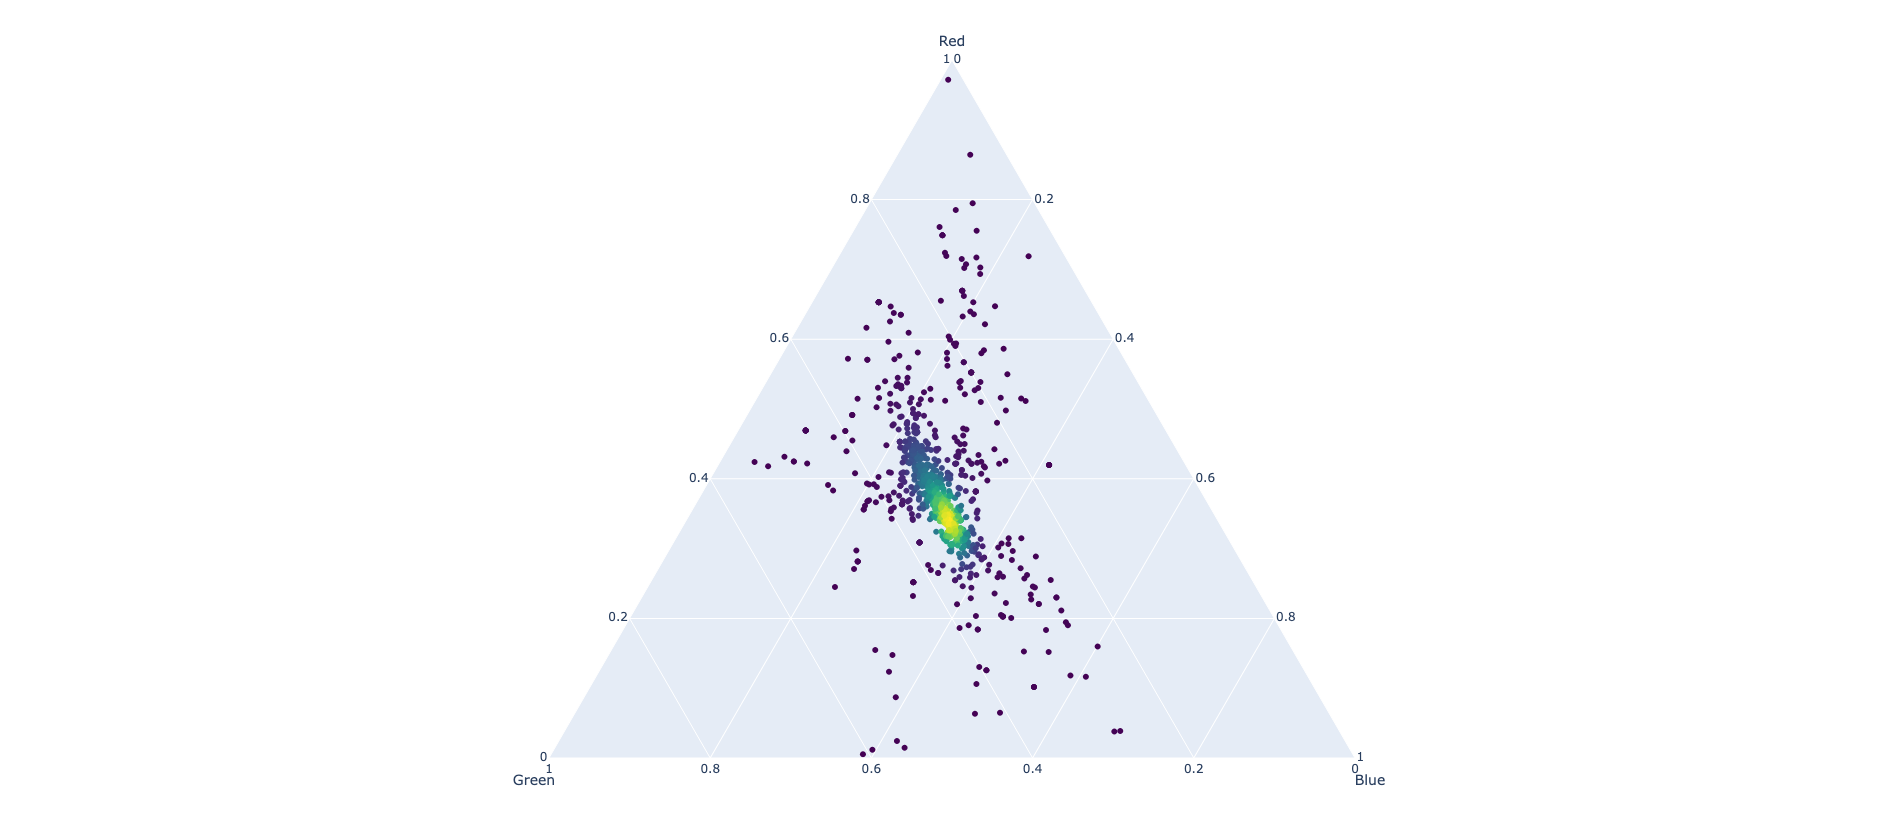
\includegraphics[width=50em,keepaspectratio]{Images/color_profile_distro.png}%
    }
    \caption{Distribution of the RGB color profiles in the dataset.}
    \label{fig:color_profile_distribution}
\end{figure}

\subsubsection{Preprocessing}

In the preprocessing phase, the RGB color representation of each image was preserved, providing three channels per pixel. Additionally, all images were rescaled to a fixed resolution of 800 × 571 pixels to eliminate size outliers. This resolution results in a total of 456,800 pixels per image, which corresponds to 1,370,400 elements when considering all three channels. The data was first transformed from an $800 \times 571 \times 3$ tensor into a $1,370,400$-element 1D vector, and the vector elements were then normalized to the range [0, 1] to standardize the input for subsequent model training. 


\subsection{Implementation Setup}
\subsubsection{Code}
\subsubsection{Memory consideration}
\subsection{Training Procedure}

\textbf{Experiment 1.}
\\	
A
\\

\textbf{Experiment 2.}
\\
A
\\

\subsection{Evaluation Metrics}

\subsubsection{loss rate}

% ============= COMPUTATIONAL ANALYSIS OF THE EXPERIMENT =============
\section{Memory Management and Information Dynamics}

% ============= FORMAL ANALYSIS OF THE MODEL =============
\section{Internal Network Rules and Formal Characterization}
Evolucion temporal, ecuaciones diferenciales parciales del entrenamiento, espacio latente en regiones de la matriz Ax y Zx

% ============= CONCLUSIONS =============
\section{Conclusions}


\subsection{Future Work}


% ============= ACKNOWLEDGMENTS =============
\section*{Acknowledgments}


% ============= REFERENCES =============
\addcontentsline{toc}{section}{References}

\begin{thebibliography}{99}

\bibitem{ejemplo2023modelo}
Pérez, J., López, M., \& García, A. (2023).
\textit{Un modelo de ejemplo para aprendizaje automático}.
Revista Latinoamericana de Ciencia de Datos, 12(3), 45--60.


\end{thebibliography}

\end{document}			